% Copyright 2004 by Till Tantau <tantau@users.sourceforge.net>.
%
% In principle, this file can be redistributed and/or modified under
% the terms of the GNU Public License, version 2.
%
% However, this file is supposed to be a template to be modified
% for your own needs. For this reason, if you use this file as a
% template and not specifically distribute it as part of a another
% package/program, I grant the extra permission to freely copy and
% modify this file as you see fit and even to delete this copyright
% notice. 

\documentclass{beamer}

% There are many different themes available for Beamer. A comprehensive
% list with examples is given here:
% http://deic.uab.es/~iblanes/beamer_gallery/index_by_theme.html
% You can uncomment the themes below if you would like to use a different
% one:
%\usetheme{AnnArbor}
%\usetheme{Antibes}
%\usetheme{Bergen}
%\usetheme{Berkeley}
%\usetheme{Berlin}
%\usetheme{Boadilla}
%\usetheme{boxes}
%\usetheme{CambridgeUS}
%\usetheme{Copenhagen}
%\usetheme{Darmstadt}
%\usetheme{default}
%\usetheme{Frankfurt}
%\usetheme{Goettingen}
%\usetheme{Hannover}
%\usetheme{Ilmenau}
%\usetheme{JuanLesPins}
%\usetheme{Luebeck}
\usetheme{Madrid}
%\usetheme{Malmoe}
%\usetheme{Marburg}
%\usetheme{Montpellier}
%\usetheme{PaloAlto}
%\usetheme{Pittsburgh}
%\usetheme{Rochester}
%\usetheme{Singapore}
%\usetheme{Szeged}
%\usetheme{Warsaw}

\usepackage{kotex}
\usepackage{braket}
\usepackage{array}
\usepackage{calc}
\usepackage{datetime}
\usepackage{dsfont}
\usepackage{amsmath}
\usepackage{listings}


\title{Lecture 4.5 : 게임이론 / Generalized Vector Space}

% A subtitle is optional and this may be deleted
\subtitle{Fastcampus Math Camp}

\author{신승우}
% - Give the names in the same order as the appear in the paper.
% - Use the \inst{?} command only if the authors have different
%   affiliation.

% \institute[Universities of Somewhere and Elsewhere] % (optional, but mostly needed)
% {
  % \inst{1}%
  % Department of Computer Science\\
  % University of Somewhere
  % \and
  % \inst{2}%
  % Department of Theoretical Philosophy\\
  % University of Elsewhere}
% - Use the \inst command only if there are several affiliations.
% - Keep it simple, no one is interested in your street address.

% - Either use conference name or its abbreviation.
% - Not really informative to the audience, more for people (including
%   yourself) who are reading the slides online

\subject{Theoretical Computer Science}

% This is only inserted into the PDF information catalog. Can be left
% out. 

% If you have a file called "university-logo-filename.xxx", where xxx
% is a graphic format that can be processed by latex or pdflatex,
% resp., then you can add a logo as follows:

% \pgfdeclareimage[height=0.5cm]{university-logo}{university-logo-filename}
% \logo{\pgfuseimage{university-logo}}

% Delete this, if you do not want the table of contents to pop up at
% the beginning of each subsection:


% \AtBeginSection[]
% {
  % \begin{frame}<beamer>{Outline}
    % \tableofcontents[currentsection,hideallsubsections]
  % \end{frame}
% }

% Let's get started
\begin{document}

\begin{frame}
 \titlepage
\end{frame}

% \begin{frame}{Outline}
  % \tableofcontents[hideallsubsections]
  % % You might wish to add the option [pausesections]
% \end{frame}

% Section and subsections will appear in the presentation overview
% and table of contents.


\section{Introduction to Game Theory} 



\subsection{Payoff Matrix and Definition of Game} 

\begin{frame}{Dice Throwing Game}

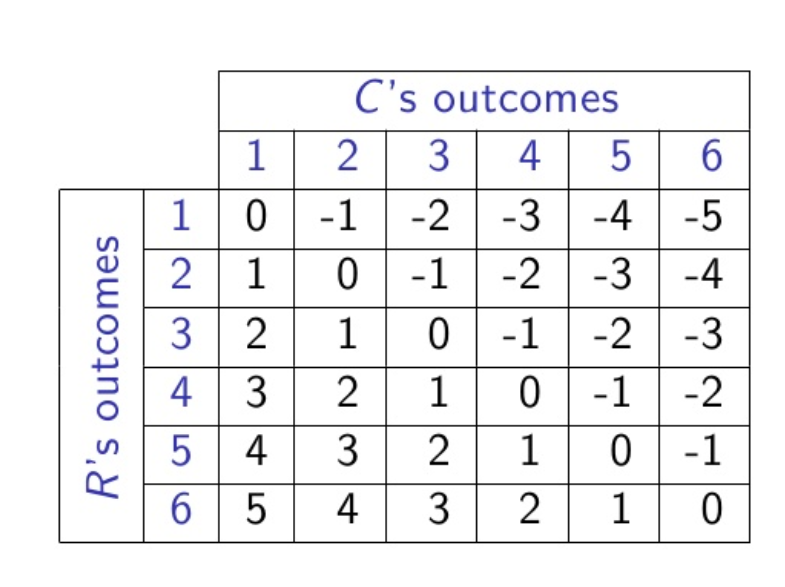
\includegraphics[width=6cm,keepaspectratio]{dice}


두 명의 플레이어 R,C가 주사위를 각자 던져서, 두 눈의 차이만큼 점수를 얻는 게임이 있다고 하자. 이 때, R이 주사위를 던져서 나온 수를 각 row에, C가 던져서 나온 수를 각 column에 대응시킨 후 교차점을 R이 얻는 점수로 하는 표를 그리면 위와 같다.  이 때, 위 표를 게임을 나타내는 행렬로 Payoff Matrix라 한다. 만약 C가 얻는 점수와 R이 얻는 점수의 합이 일정하다면, 이러한 게임을 제로섬 게임이라고 한다. 

\end{frame} 


\begin{frame}{Expected Value}
이 때, 플레이어 R이 선택할 수 있는 옵션과 그 각각에 대한 확률을 row vector, C는 column vector으로 나타내자. 그러면 다음과 같이 쓸 수 있다. 

\begin{eqnarray} 
\vec{p}& = &\left[ \begin{matrix} p_1 & p_2 & ... & p_n \end{matrix} \right] \\
\vec{q}& = &\left[ \begin{matrix} q_1 \\ q_2 \\ ... \\ q_n \end{matrix} \right]
\end{eqnarray}
 
이 때, Payoff Matrix를 A라고 할 때, R이 얻는 점수의 기댓값은 $E(\vec{p}, \vec{q}) = \vec{p}A\vec{q}$라고 볼 수 있다. 
\end{frame} 


\begin{frame}{Expected Value : Fair Dice}
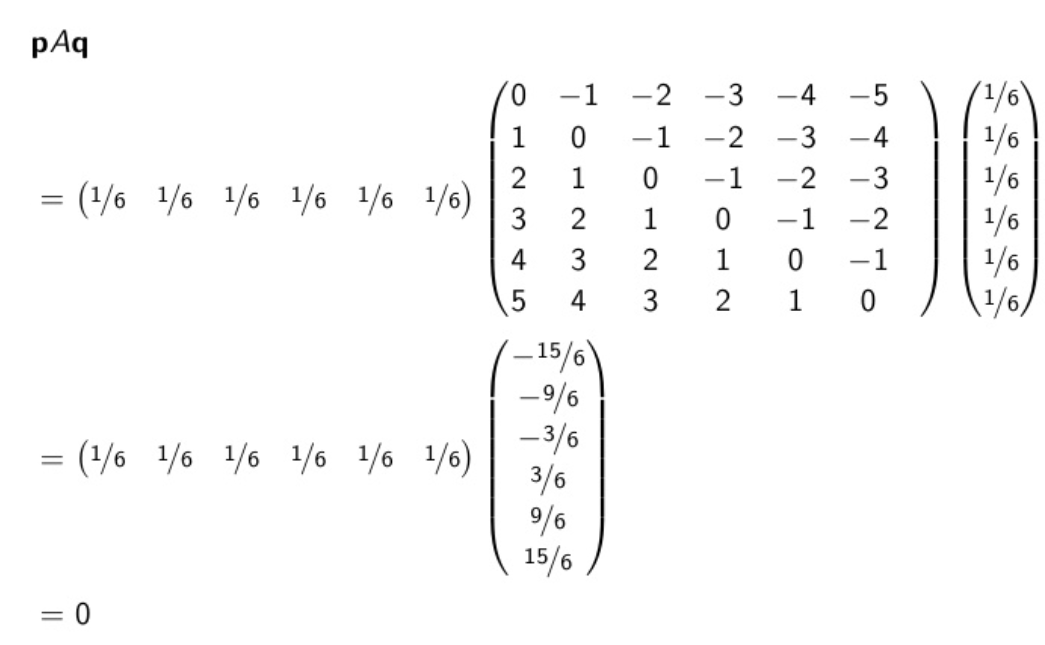
\includegraphics[width=10cm,keepaspectratio]{fair}
\end{frame} 


\begin{frame}{Expeced Value : Unfair Dice}

만약 R이 던지는 주사위가 조작되어 있어서, 확률이 균등하게 $\frac{1}{6}$이 아니라 $(1/10 1/10 1/5 1/5 1/5 1/5)$라고 해 보자. 그러면 기대값은 아래와 같이 바뀐다. 
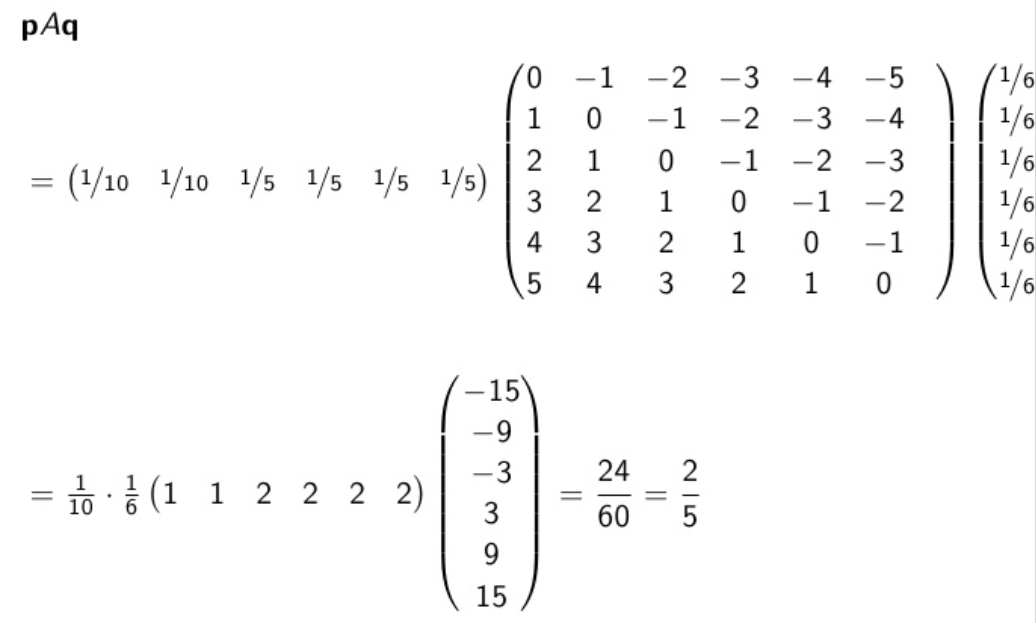
\includegraphics[width=10cm,keepaspectratio]{unfair}

\end{frame} 


\begin{frame}{Strategy Profile}
여기서, 위에서 나온 벡터 $\vec{p}, \vec{q}$를 Strategy Profile이라고 한다. 

\begin{itemize} 
\item strategy profile의 원소의 합은 1이다. 
\item  strategy profile이 1과 0으로만 이루어져 있다면, pure strategy라고 한다. 그렇지 않으면 mixed strategy라고 한다. 
\end{itemize}

\end{frame} 


\subsection{Nash Equilibrium} 

\begin{frame}{Finding Equilibrium : min-max}
위에서 언급된 게임에서, 모든 가능한 strategy profile들 $\vec{p}, \vec{q}$에 대해서 다음이 성립하는 $\vec{p*}, \vec{q*}$가 항상 존재한다. 

\begin{equation} 
E(\vec{p*}, \vec{q}) \leq E(\vec{p*}, \vec{q*}) \leq E(\vec{p}, \vec{q*}) 
\end{equation}

이 때, $E(\vec{p*}, \vec{q*})$를 게임의 값(value)라고 하며, 양자는 그러한 $\vec{p*}, \vec{q*}$를 선택하게 된다. 이를 내쉬 균형이라 한다. 

예시를 들어서 살펴보자. 우선, p와 q가 pure strategy인 경우 두 가지를 먼저 살펴보자. 
\end{frame} 

\begin{frame}{Dice Game Revisited}
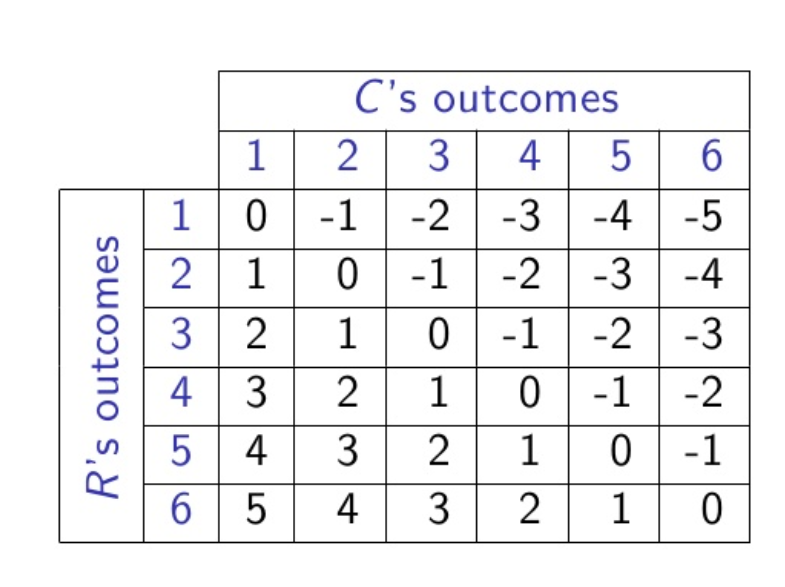
\includegraphics[width=6cm,keepaspectratio]{dice}

만약 위 주사위 게임에서, R과 C가 각자 원하는 대로 주사위를 조작해서 게임이 임한다고 가정하자. 그렇다면 둘 모두 6만 나오는 주사위를 가지고 게임할 것이다. 이를 앞에서 언급한 슬라이드를 이용하여 생각해 보자. 

\end{frame}

\begin{frame}{Broadcasting Station }
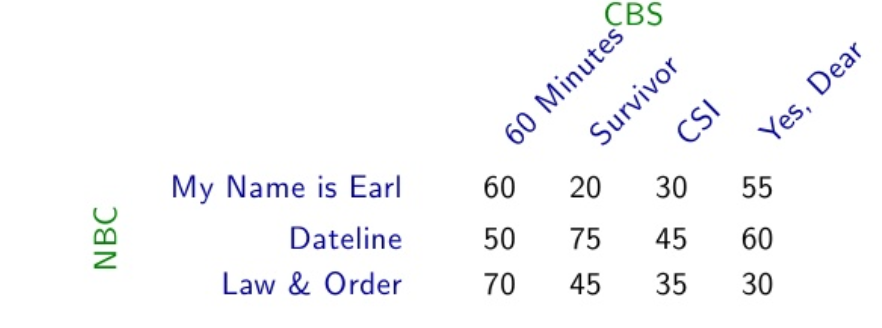
\includegraphics[width=10cm,keepaspectratio]{broad}

위와 같은 경우, 각 숫자는 R, 즉 여기서는 NBC의 시청율이라고 하자. 이 때, NBC와 CBS가 선택할 방영 프로그램은 무엇일지 생각해 보자. 

\end{frame}




\begin{frame}{Broadcasting Station }
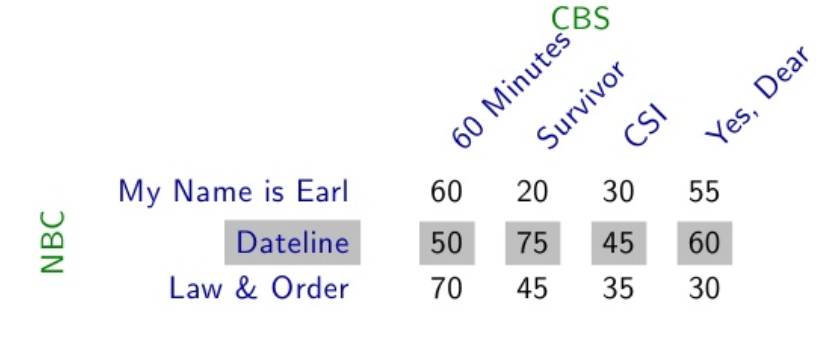
\includegraphics[width=10cm,keepaspectratio]{dateline}

먼저, NBC의 경우 NBC가 얻을 최소값을 최대화하고 싶어한다고 생각하자. (min-max)
이 때, 선택할 수 있는 전략은 Dateline을 방영하는 것이다. 

\end{frame}


\begin{frame}{Broadcasting Station }
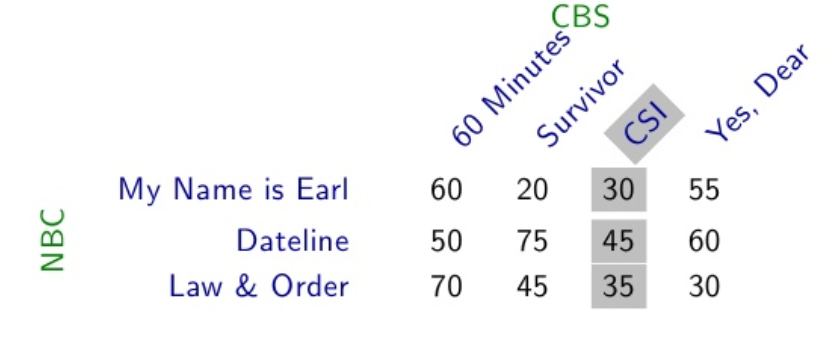
\includegraphics[width=10cm,keepaspectratio]{csi}

CBS의 경우 NBC가 얻을 최댓값을 최소화하고 싶어한다고 생각하자. (max-min)
이 때, 선택할 수 있는 전략은 CSI를 방영하는 것이다. 이와 같이 고르면 '안전한' 선택을 하는 것으로 보인다. 이것이 정말 최적일까? 

\end{frame}

\begin{frame}{Broadcasting Station }
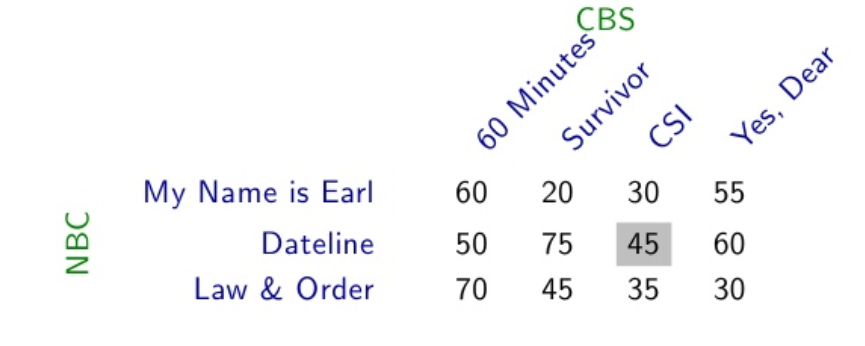
\includegraphics[width=10cm,keepaspectratio]{eq}

이 경우, 양자는 암묵적으로 (Dateline, CSI)에 합의하게 되며, 그렇게 방영할 경우 양자의 이득이 극대화된다고 판단할 것이다. 즉, 양자 중 다른 한 사람이 전략을 변화시키지 않으면, 다른 사람도 전략을 변화시키지 않을 것이다. 이런 경우를 stable한 내쉬 균형이라고 한다. 반대로, 그 점에서 한 사람이 조금 전략을 변형시킬 때 양자의 전략이 극단적으로 변한다면 이러한 내쉬 균형을 unstable한 내쉬 균형이라고 한다. 
\end{frame}




\begin{frame}
위와 같은 식으로 고를 때, 최적이 됨을 증명하자. 즉, 

\begin{equation} 
E(\vec{p*}, \vec{q}) \leq E(\vec{p*}, \vec{q*}) \leq E(\vec{p}, \vec{q*}) 
\end{equation}

임을 증명하자. 

가정에 따라서  $\vec{p*}, \vec{q*}$은 각각 pure strategy로, $\vec{e_r}, \vec{e_s}$로 볼 수 있다. 그러면, 위와 같이 $\vec{e_r}, \vec{e_s}$를 고르는 것은 곧 $\forall j a_{rj} \leq a_{rs}, \forall i a_{is} \geq a_{rs}$를 고르는 것이다. 


\begin{equation} 
E(\vec{e_r}, \vec{q}) = \vec{e_r}A\vec{q} \leq a_{rs} = E(\vec{e_r}, \vec{e_s})
\end{equation}

또, 비슷하게 

\begin{equation} 
E(\vec{e_r}, \vec{q}) = \vec{e_r}A\vec{q} \leq a_{rs} = E(\vec{e_r}, \vec{e_s})
\end{equation}

이다. 따라서 최적해가 된다. 


\end{frame}



\begin{frame}{Finding Equilibrium : general case}

2 player, 2 options : 2-vector $\vec{p}, \vec{q}$ 와 2 by 2 행렬 A에 대해서, 

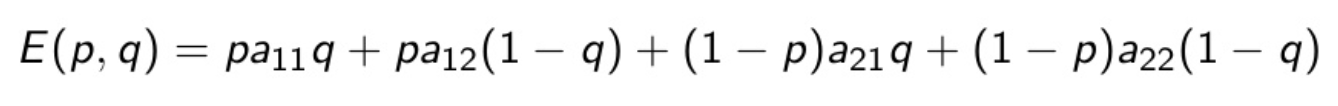
\includegraphics[width=10cm,keepaspectratio]{exp}

이 때 극점은 각각 

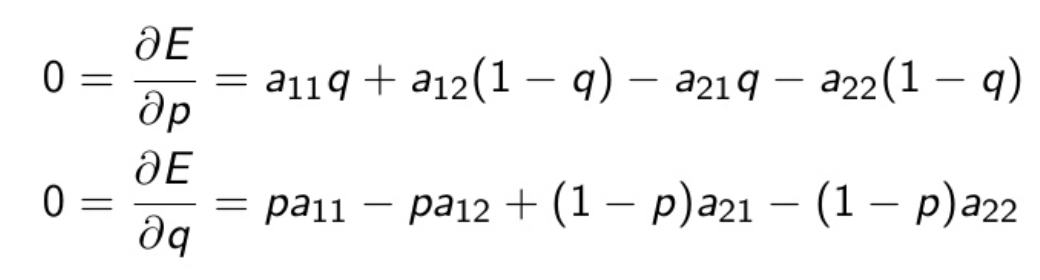
\includegraphics[width=10cm,keepaspectratio]{crit}

으로 구할 수 있다. 
\end{frame} 


\begin{frame}{Chicken Game} 
2차선에서 각자 반대 방향으로 달리는 차가 있다. 이 때, 이들 간 payoff matrix는 둘이 같은 도로를 고를 경우 0, 다른 도로를 고를 경우 1이다. 이 때, 가능한 내쉬균형을 모두 구해보자. 
\end{frame}


\begin{frame}{Wardrop Model}

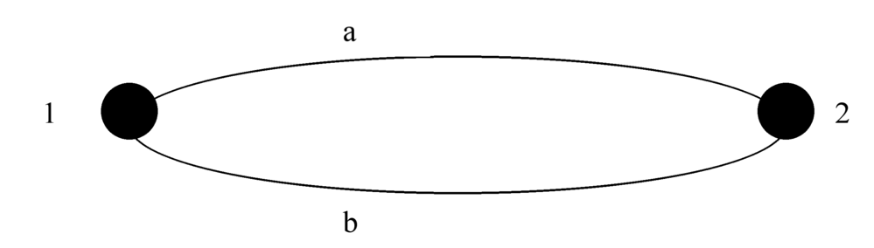
\includegraphics[width=10cm,keepaspectratio]{wardrop}

\end{frame} 







\section{Generalized Vector}


\begin{frame}{Generalized Arithematic Operations} 

이때까지 벡터, 행렬 등의 \textit{선형대수학적} 객체들의 더하기와 상수배의 operation에 대해서 다루었다. 이제 이 연산을 확장해 보자. 즉, 이제부터는 더하기, 곱하기 등은 굳이 사칙연산일 필요가 없다. 예컨대, 함수끼리의 곱셈을 다음과 같이 정의할 수도 있다. 

$\int f \bullet g dx $ 

더하기 역시 정의하기 나름이다. 이제부터 이러한 일반화된 사칙연산을 고려하기 위한 체계를 세워보겠다. 

\end{frame}

% \begin{frame}{Field} 

% Field는 집합 하나와 그 집합의 원소간의 6개의 연산으로 정의된다. 

% \begin{itemize} 
% \item binary 연산 2개 : 더하기/곱하기 
% \item unary 연산 2개 : 덧셈의 역원/곱셈의 역원 
% \item constant 연산 2개 : 덧셈의 항등원(0) / 곱셈의 항등원(1)
% \end{itemize}

% 이 때, binary 연산은 교환법칙과 결합법칙이 성립해야 하며, 연산의 결과는 언제나 집합의 원소여야만 한다. 

% \end{frame}

\begin{frame}{항등원과 역원} 
어떤 집합 S에서의 이항연산 f에 대해서, 

\begin{itemize} 
\item 집합 S의 모든 원소 s에 대해서 f(s,i) = f(i,s) = s 이면 i를 그 연산의 항등원이라고 한다. 
\item 집합 S의 어떤 원소 s에 대해서 f(s, t) = f(t, s) = i 이면 t를 s의 역원이라고 한다. 
\end{itemize}
\end{frame}

\begin{frame}{Generalized Vector Space} 

어떤 집합 F 위에서 정의된 벡터공간 V는 어떤 집합 V와 F의 원소 a,b 와 V의 원소 $\vec{v}, \vec{u}$에 대해서 다음이 성립하는 벡터연산 더하기와 스칼라곱, 그리고 덧셈의 역원으로 정의된다. 이 때, F를 이 벡터공간의 스칼라라고 한다. 

\begin{itemize} 
\item 벡터덧셈의 교환법칙 / 결합법칙 
\item 벡터덧셈의 항등원 / 역원
\item 스칼라의 곱셈에서의 항등원 1에 대해서, $1\vec{v} = \vec{v}$
\item $(ab)\vec{v} = a(b\vec{v})$ 
\item $a(\vec{v} + \vec{u}) = a\vec{v} + a\vec{u} $
\item $(a+b)\vec{v} = a\vec{v} + b\vec{v}$
\end{itemize}

여기서, 스칼라곱과 벡터-스칼라곱이나 스칼라끼리의 합과 벡터-벡터간의 합은 다른 operation이다. 

\end{frame}

% https://math.okstate.edu/people/binegar/3013-S99/3013-l12.pdf
\begin{frame}{Examples of an Abstract Vector Space} 
\begin{itemize} 
\item Polynomials with degree $\leq n$
\item Matrices
\item Linear Transformations
\item Functions from a specific domain (will be revisited after few weeks)
\item Random Variables (will be revisited after few weeks)
\end{itemize}
\end{frame}

\begin{frame}{예시 : $\mathds{R}^2$에서 $\mathds{R}^2$로의 선형변환}

$\mathds{R}^2$에서 $\mathds{R}^2$로의 선형변환은 2 by 2 행렬로 나타내어질 수 있다. 따라서, 행렬의 덧셈과 실수배를 이용하여 선형변환의 벡터공간을 정의할 수 있다. 이제부터 이 공간의 기저와 좌표, 그리고 2차원 좌표계에서 선형변환 벡터들이 어떠한 의미를 가지는지를 알아볼 것이다. 

\end{frame}

\begin{frame}{예시 : $\mathds{R}^2$에서 $\mathds{R}^2$로의 선형변환} 
먼저, 다음의 행렬들을 생각해 보자. 
$ \vec{e}_1 =  
\left[ \begin{matrix}
1 & 0  \\
0 & 0 
\end{matrix} \right],
\vec{e}_2 = 
\left[ \begin{matrix}
0 & 1  \\
0 & 0 
\end{matrix} \right],
\vec{e}_3 = 
\left[ \begin{matrix}
0 & 0  \\
1 & 0 
\end{matrix} \right],
\vec{e}_3 = 
\left[ \begin{matrix}
0 & 0  \\
0 & 1 
\end{matrix} \right]
$

이 행렬들은 명백하게 2 by 2 행렬이므로, $\mathds{R}^2$에서 $\mathds{R}^2$로의 선형변환이다. 이들 벡터는 선형독립일까? 또, 위 4개의 벡터는 기저가 될까? 
\end{frame}

\begin{frame}{Linear Independence of an Abstract Vector Space}
위 4개의 벡터가 선형독립이기 위해서는 $c_ie_i$을 만족하는 $c_i$가 0뿐이여야 한다. 위 경우, 

$c_i\vec{e}_i = \left[ \begin{matrix}
c_1 & c_2  \\
c_3 & c_4 
\end{matrix} \right]$ 이므로 선형독립임을 알 수 있다. 

또한, 임의의 2 by 2 행렬을 $c_i$를 적절히 조정하여 만들 수 있으므로, 기저임을 알 수 있다. 
\end{frame}



\begin{frame}{예시 : $\mathds{R}^2$에서 $\mathds{R}^2$로의 선형변환} 

위와 같이 선형변환의 기저를 찾은 것은 어떤 의미가 있을까? 

이는 이제부터 우리가 $\mathds{R}^2$의 한 점에서 $\mathds{R}^2$의 한 점으로 대응시키는 선형변환을 언제나 4개의 선형변환을 조합하여 하는 것으로 이해할 수 있다는 점이다. 
\end{frame}


% \begin{frame}{Extending an Abstract Vector Space : Inner Product Space} 
% 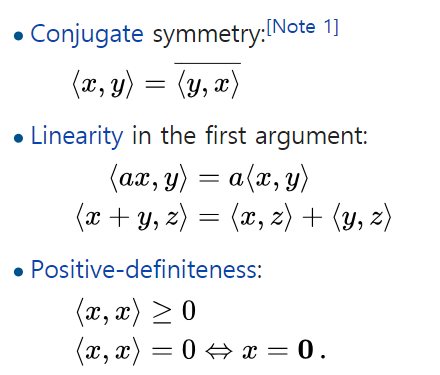
\includegraphics[width=10cm,keepaspectratio]{innerproduct}
% \end{frame}











\end{document}


